% -*- latex -*-
%%%%%%%%%%%%%%%%%%%%%%%%%%%%%%%%%%%%%%%%%%%%%%%%%%%%%%%%%%%%%%%%
%%%%
%%%% This TeX file is part of the course
%%%% Introduction to Scientific Programming in C++/Fortran2003
%%%% copyright 2017-2022 Victor Eijkhout eijkhout@tacc.utexas.edu
%%%%
%%%% structf.tex : types Fortran
%%%%
%%%%%%%%%%%%%%%%%%%%%%%%%%%%%%%%%%%%%%%%%%%%%%%%%%%%%%%%%%%%%%%%

Fortran has structures for bundling up data, but there is no
\n{struct} keyword: instead you declare both the structure type and
variables of that \indextermsub{derived}{type} with the 
\indexfdef{type} keyword. 

\Level 0 {Derived type basics}

\begin{slide}{Structures: \noexpand\texttt{type}}
  \label{sl:ftype}
  \begin{itemize}
  \item Fortran has structures similar to~C:\\
    bundle variables --~of different types.
  \item Structures are a \indextermsub{derived}{type}: you can create
    variables of that type, but it's not a built-in type.
  \item  Fortran keyword for derived types is (confusingly) \indexf{Type}
  \end{itemize}
\end{slide}

Now you need to
\begin{itemize}
\item Define the type to describe what's in it;
\item Declare variables of that type; and
\item use those variables, but setting the type members or using their
  values.
\end{itemize}

\begin{block}{Type declaration}
  \label{sl:ftype-def}
  \lstinline{Type name} / \lstinline{End Type name} block.\\
  Member declarations inside the block:
\begin{lstlisting}
type mytype
  integer :: number
  character :: name
  real(4) :: value
end type mytype
\end{lstlisting}
  Type definitions go before executable statements.
\end{block}

Creating type variables is a little different from
objects in a ~C++ class.
In C++ the class name could be used by itself
as the datatype; in Fortran you need to write
\lstinline{Type(mytype)}.
Otherwise, it looks like any other variable declaration.

\begin{block}{Creating / initializing type variables}
  \label{sl:ftype-set}
  Declare type variables in the main program:
\begin{lstlisting}
Type(mytype) :: struct1,struct2
\end{lstlisting}
 Initialize with type name:
\begin{lstlisting}
struct1 = mytype( 1, 'my_name', 3.7 )
\end{lstlisting}
Copying:
\begin{lstlisting}
struct2 = struct1
\end{lstlisting}
\end{block}

If you need access to a single field in a type, 
there is a notation analogous to the `dot' notation in~C++:
in Fortran you use the percent sign~\verb+%+.

\begin{block}{Member access}
  \label{sl:ftype-access}
  Access structure members with \verb+%+\\
  (compare C++ dot-notation)
\begin{lstlisting}
Type(mytype) :: typed_struct
typed_struct%member = ....  
\end{lstlisting}
\end{block}

As an example, we use the `point' structure
from the geometry project.

\begin{block}{Example}
  \label{sl:ftype-ex}
  \begin{multicols}{2}
    \verbatimsnippet{ftypedef}
    \columnbreak
    \verbatimsnippet{ftypeuse}
  \end{multicols}
\end{block}

Note that printing a type by itself is equivalent to printing
its components in sequence.

You can have arrays of types:
\begin{lstlisting}
type(my_struct) :: data
type(my_struct),dimension(10) :: data_array
\end{lstlisting}

\Level 0 {Derived types and procedures}

\begin{block}{Structures as procedure argument}
  \label{sl:ftype-pass}
  Structures can be passed as procedure argument, just like any other
  datatype. In this example the function \lstinline{length}:
  \begin{itemize}
  \item Takes a structure of \lstinline{type(point)} as argument; and
  \item returns a \lstinline{real(4)} result.
  \item The structure is declared as \lstinline{intent(in)}.
  \end{itemize}

  \begin{multicols}{2}
    Function with structure argument:
    \verbatimsnippet{ftypepass}
    \columnbreak
    Function call
    \verbatimsnippet{ftypecall}
  \end{multicols}
\end{block}

\begin{exercise}
  \label{ex:ftype-angle}
  Add a function \lstinline{angle} that takes a \lstinline{Point}
  argument and returns the angle of the $x$-axis and the line
  from the origin to that point.

  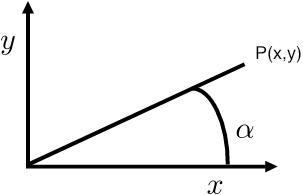
\includegraphics[scale=.3]{pointangle}

  Your program should read in the $x,y$ values of the point
  and print out the angle in radians.

  Bonus: can you print the angle
  as a fraction of~$\pi$? So
  \[ (1,1) \Rightarrow 0.25 \]
  \skeleton{point}
\end{exercise}

\begin{exercise}
  \label{ex:ftype-rect}
  Write a program that has the following:
  \begin{itemize}
  \item A type \lstinline{Point} that contains real numbers~\lstinline{x,y};
  \item a type \lstinline{Rectangle} that contains two \lstinline{Point}s,
    corresponding to the lower left and upper right point;
  \item a function \lstinline{area} that has one argument: a \lstinline{Rectangle}.
  \end{itemize}
  Your program should
  \begin{itemize}
  \item Accept two real numbers on one line, for the bottom left point;
  \item similarly, again on one line, the coordinates of the top right point; then
  \item print out the area of the (axi-parallel) rectangle defined by these two points.
  \end{itemize}
\end{exercise}

\begin{exercise}
  In the previous exercise~\ref{ex:ftype-rect}:\\
  Bonus points for using a module,\\
  double bonus points for using an object-oriented solution.
\end{exercise}

\Level 0 {Parametrized types}

If a derived type contains an array,
you may want to have the length of that array
to be variable, without making the array dynamically allocatable.
For this, Fortran has \indextermdef{parametrized}{type}s:
you can define a type with some combination of:
\begin{itemize}
\item a parameter with attribute \indexf{len},
  used as the length of an array member; or
\item a parameter with attributute \indexf{kind},
  used as the kind of some variable; section~\ref{sec:fprecision}.
\end{itemize}

Example:
\verbatimsnippet{ftypedefd}

I haven't figured out how to set variables:
\verbatimsnippet{ftypeused}

These types can be passed normally:
\verbatimsnippet{ftypepassd}
